\documentclass{article}
\usepackage[utf8]{inputenc}
\usepackage[T1]{fontenc}
\usepackage[a4paper]{geometry}
\usepackage{amsmath}
\usepackage{amssymb}
\usepackage{graphicx}
\usepackage{rotating}
\usepackage{placeins}
\usepackage[slovak]{babel}
\usepackage{makeidx}
\usepackage[colorlinks=true,linkcolor=blue,urlcolor=black]{hyperref}
\usepackage{bookmark}

\renewcommand{\figurename}{Obr.}
\renewcommand{\tablename}{Tab.}
\newcommand{\overbar}[1]{\mkern 1.5mu\overline{\mkern-1.5mu#1\mkern-1.5mu}\mkern 1.5mu}

\makeindex


\begin{document}
	\title{ Semestrálny projekt Osciloskop - špecifikácia }
	\author{Denis Vasko a Ján Urdianyk} 
	\maketitle
	\thispagestyle{empty}
	\section{Špecifikácia}
	Napätie na kanáloch chceme vzorkovať s pevnou periódou. Hodnoty budeme zapisovať do pamäťového buffra cez DMA. Vzorky sa budú prepočítavať podľa nastavení osciloskopu v pamäti mikropočítača(Vertikálny posun, horizontálny posun, vertikálne škálovanie atď.). Prepočítané vzorky sa potom pošlú do GUI na PC cez perifériu USART, kde sa vykreslí priebeh napätí. Nastavenie osciloskopu budeme meniť cez GUI pri zmene sa pošlú nové nastavenia do mikropočítača cez sériovú linku.
\section{Funkcie osciloskopu}
\begin{itemize}
	\item Meracia mriežka (Graticule) 
	\item Ovládanie časovej základne - čas/horizontálny diel
	\item Vertikálne škálovanie - škálovanie konštantou, zmena polarity
	\item X-Y mód (vykreslenie závislosti napätia na kanále Y od napätia na kanále X)
	\item Horizontálne škálovanie - pre X-kanál v X-Y móde
	\item Vertikálny posun - pre oba kanály zvlášť
	\item Horizontálny posun - pre oba kanály zvlášť
	\item Možnosť zobrazenia časového priebehu napätí na oboch kanáloch zároveň (Prepínanie len Y, len X, oba X aj Y alebo X-Y mód)
	%\item Tigrovaný vstup - štart zobrazenia pri dosiahnutí dostatočnej úrovne napätia na sledovanom/ných kanáloch
	%\item Hold-off - po trigrovaní vstupu sa ďalšie vykreslenie nemôže uskutočniť kým neprejde daný čas - cooldown trigrovania
	%\item Automatické prekresľovanie - aj keď napätie na kanály nedosiahne dostatočnú hodnotu na trigoravnie, aj tak sa periodicky kanál prekresľuje s istou periódou. V prípade, že napätie na kanály dosiahne trigrovacie napätie, automatické prekresľovanie sa vypne (restne sa časovač), potom sa znovu zapne po neprítomnosti trigrovacieho napätia na kanály
	\item Jednorázové vykreslenie - vykreslenie jedného merania 
	\begin{itemize}
		\item štart merania pri presiahnutí úrovne napätia
	%	\item štart po istom čase 
	\end{itemize}
\end{itemize} 
\section{Náčrt štruktúry programu}

\begin{figure}[!h]
	\centering
	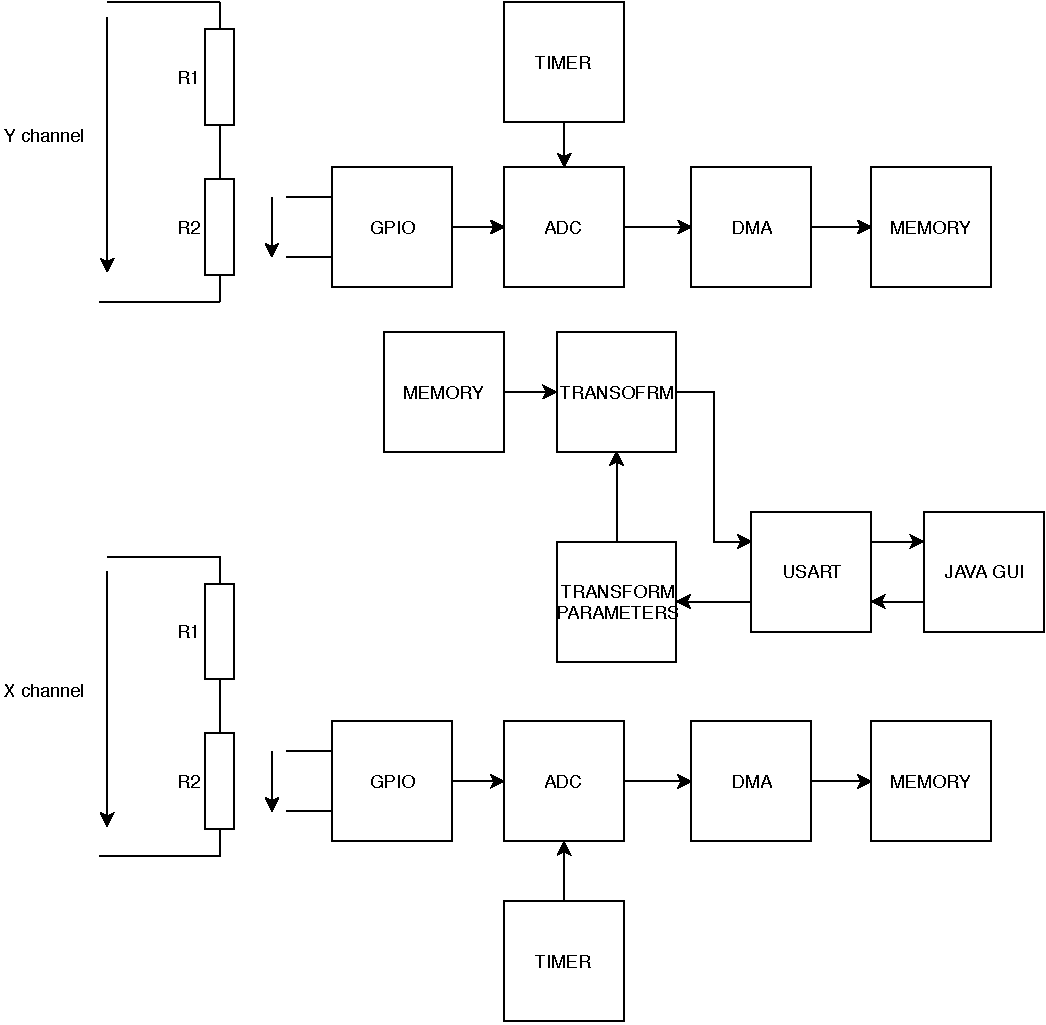
\includegraphics[width=\linewidth]{../Obrazky/basicstructure.pdf}
\end{figure}
	
	
	%\printindex
\end{document}
